%==================================================================%
% Author : Pando Muñoz, Manuel                                     %
% Sánchez Barreiro, Pablo                                          %
% Version: 1.0, 02/03/2011                                         %
%                                                                  %
% Memoria del Proyecto Fin de Carrera                              %
% Archivo raíz para el capítulo de iteración1                      %
%==================================================================%

\chapterheader{Creación del sistema distribuido base}{Creación del sistema distribuido base}
\label{chap:iteracion1}


En el siguiente capítulo se describe lo realizado en la primera iteración de la fase de construcción.
\newline


La base de la que se parte son los resultados de las iteraciones anteriores, correspondientes a las fases de iniciación y elaboración, es decir, los requisitos del sistema y su arquitectura.
\newline

De acuerdo con lo planificado en la sección \ref{sec:planificacion:iteraciones}, el objetivo de esta iteración es el de crear la base del sistema distribuido, implementando los requisitos de la tabla \ref{tabla:iteracion1:requisitosObjetivo} que son el subconjunto de los casos de uso mostrados en la figura \ref{fig:iteracion1:casosUso}.
\newline

El primer paso en una iteración de la fase de construcción de acuerdo a la metodología es refinar los requisitos de alto nivel a implementar, con lo que obtenemos la tabla \ref{tabla:iteracion1:requisitosObjetivoRefinados}
\newline


\chaptertoc


\begin{table}
    \begin{tabular}{|c|p{12cm}|}
        \hline
        \textbf{Identificador} & \textbf{Descripción}
        \\ \hline

        R01 & Un computador de la red debe poder ser designado como \emph{Watchman}.
        \\ \hline

        R02 & Todos los computadores que no sean \emph{Watchman} serán computadores
        normales, y podrán ser utilizados para la realización de las pruebas evaluables.
        \\ \hline

        R06 & El profesor debe ser capaz desde el \emph{Watchman} de enviar el fichero de enunciado al resto de computadores.
        \\ \hline

        R07 & El alumno desde su computador debe ser capaz de conectarse al \emph{Watchman}.
        \\ \hline

        R13 & La aplicación ha de ser capaz de comprobar que los archivos se han enviado correctamente.
        \\ \hline

    \end{tabular}
    \caption{Requisitos objetivo de la iteración}
    \label{tabla:iteracion1:requisitosObjetivo}
\end{table}


\begin{table}
    \begin{tabular}{|c|p{12cm}|}
        \hline
        \textbf{Identificador} & \textbf{Descripción}
        \\ \hline

        R01 & Un computador de la red debe poder ser designado como \emph{Watchman}.
        \\ \hline

        R02 & Todos los computadores que no sean \emph{Watchman} serán computadores
        normales, y podrán ser utilizados para la realización de las pruebas evaluables.
        \\ \hline

        R06 & El profesor debe ser capaz desde el \emph{Watchman} de enviar el fichero de enunciado al resto de computadores.
        \\ \hline

        R06.1 & El profesor escogerá el fichero a enviar con un diálogo desde la aplicación.
        \\ \hline

        R06.2 & Solamente es posible transferir un fichero a la vez.
        \\ \hline

        R07 & El alumno desde su computador debe ser capaz de conectarse al \emph{Watchman}.
        \\ \hline

        R07.1 & La identificación del equipo necesaria para la conexión del \emph{Watchman} se realizará por medio de la IP.
        \\ \hline

        R07.2 & El \emph{Watchman} debe soportar conexiones simultáneas.
        \\ \hline

        R07.3 & Para una correcta conexión son necesarios datos del alumno, nombre y apellidos.
        \\ \hline

        R07.4 & Para una correcta conexión es necesario que el alumno indique en que directorio desea recibir el enunciado en caso de que lo haya.
        \\ \hline

        R07.4.1 & El alumno ha de tener permisos de escritura en el directorio que seleccione.
        \\ \hline

        R13 & La aplicación ha de ser capaz de comprobar que los archivos se han enviado correctamente.
        \\ \hline

        R13.1 & Para la comprobación de integridad de los archivos se usarán firmas MD5.
        \\ \hline

    \end{tabular}
    \caption{Requisitos objetivo refinados de la iteración}
    \label{tabla:iteracion1:requisitosObjetivoRefinados}
\end{table}


\begin{figure}[]
    \centering
    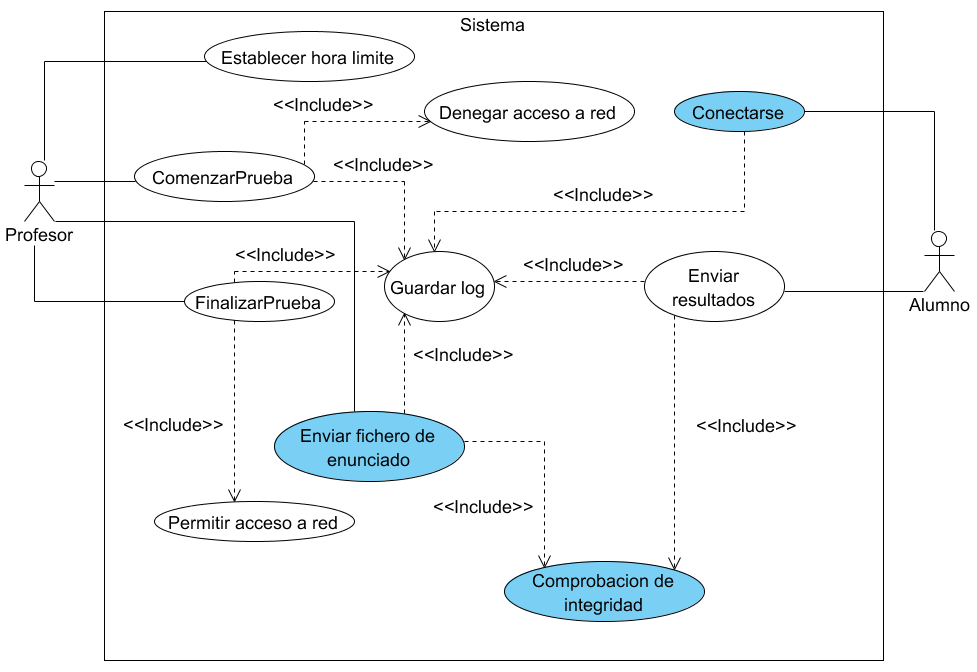
\includegraphics[width=.90\linewidth]{iteracion1/casosUso}
    \caption{Casos de uso a implementar}
    \label{fig:iteracion1:casosUso}
\end{figure}


\section{Incrementos realizados}

En las siguientes secciones se describen los incrementos realizados para la implementación.


\subsection{Interfaces gráficas}

Los requisitos R01 y R02 no reflejan funcionalidades que ha de tener el sistema, sino que tratan sobre la arquitectura del mismo. Como se ha comentado es un software distribuido, así que tenemos dos aplicaciones distintas. Las interfaces diseñadas para estas aplicaciones se muestran en la imagen \ref{fig:iteracion1:GUIProf} la que utilizará el profesor y en la \ref{fig:iteracion1:GUIAlu} la que utilizará el alumno.
\newline


\begin{figure}
    \centering
    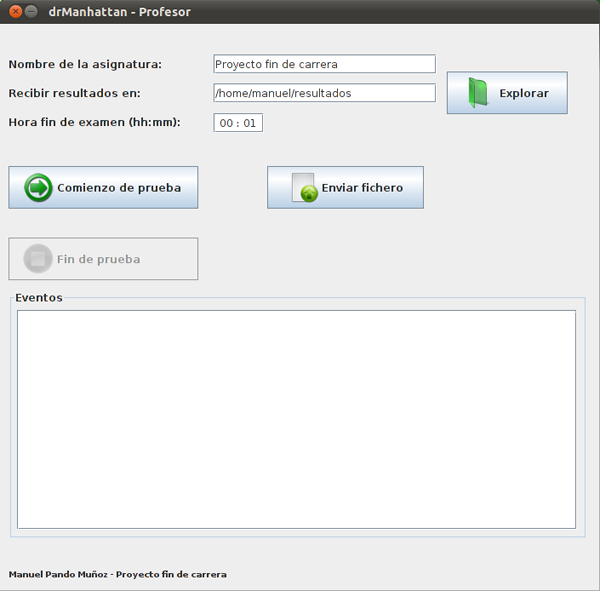
\includegraphics[width=.90\linewidth]{iteracion1/GUIProfesor}
    \caption{Interfaz de la aplicación profesor}
    \label{fig:iteracion1:GUIProf}
\end{figure}


\begin{figure}
    \centering
    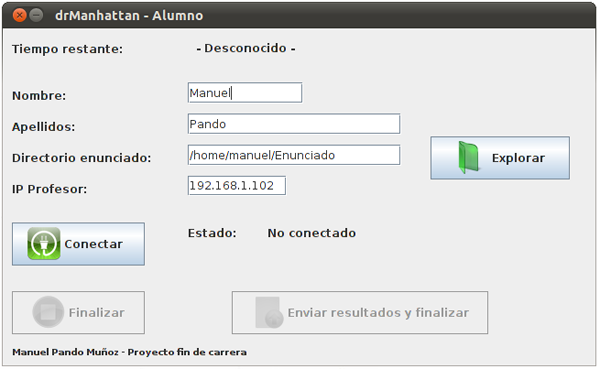
\includegraphics[width=.90\linewidth]{iteracion1/GUIAlumno}
    \caption{Interfaz de la aplicación alumno}
    \label{fig:iteracion1:GUIAlu}
\end{figure}



\subsection{Conexión}
\label{sec:iteracion1:conexion}

En esta sección se comenta el proceso para implementar el requisito R07 \lq \lq El alumno desde su computador debe ser capaz de conectarse al \emph{Watchman}\rq \rq \ el caso de uso \lq \lq Conectarse\rq \rq \ representado en el diagrama de secuencia de la imagen \ref{fig:iteracion1:casosUso}. El resto de diagramas de cada caso de uso se encuentran en el CD, en la carpeta UML.
\newline

\begin{figure}
    \centering
    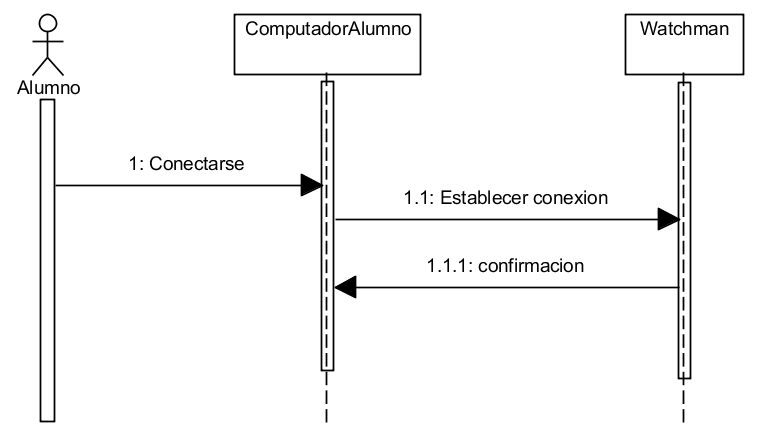
\includegraphics[width=.90\linewidth]{iteracion1/secConectar}
    \caption{Diagrama de secuencia caso de uso conectar}
    \label{fig:iteracion1:casosUso}
\end{figure}

En este incremento la aplicación del alumno debe, dada la IP del equipo dónde se está ejecutando el computador del profesor, establecer una conexión con él. Este es un punto básico del sistema, si no se es capaz de establecer correctamente una conexión, las dos aplicaciones no podrán comunicarse y no funcionará nada.
\newline

Para que se pueda establecer la conexión se utilizan las clases \lq \lq ServerSocket\rq \rq \  y \lq \lq Socket\rq \rq, de la librería \lq \lq java.net\rq \rq\cite{JAVA:1998, JAVANET:2010}. Con la primera conseguimos que la aplicación del profesor espere nuevas conexiones de alumnos y con la segunda creamos realmente la conexión desde la aplicación del alumno, partiendo de la IP proporcionada. Cada vez que se crea una conexión nueva se almacena en una lista. Además, como no se quiere bloquear la interfaz gráfica\cite{GUI:1999} del profesor mientras los alumnos se conectan, esto se realiza en un hilo de ejecución\cite{THREAD:2004} aparte.


\subsection{Envío de ficheros}
\label{sec:iteracion1:envio}

Una vez que los alumnos están conectados correctamente el profesor puede enviarles un enunciado o ficheros necesarios para la realización de la prueba y el sistema ha de poder detectar errores en la transferencia de dichos ficheros. Como ya hemos comentado, la aplicación del profesor mantiene una lista con la conexiones creadas de modo que leer un fichero y enviarlo por cada conexión de la lista es un proceso trivial.
\newline


\section{Pruebas}
\label{sec:iteracion1:pruebas}

Después de finalizar la codificación de las funcionalidades descritas en las secciones anteriores es el turno para las pruebas.
\newline

Debido a la naturaleza del sistema, automatizar pruebas con una herramienta estilo \emph{JUnit} se antoja difícil, ya que funciona a base de eventos\cite{EVENTOS:2010} y es distribuido, por eso, para probar la aplicación se utilizan secuencias de acciones con el fin de desencadenar los eventos requeridos en cada funcionalidad. En esta iteración se realizan las siguientes:

\begin{itemize}


    \item {\bfseries R07} El alumno desde su computador debe ser capaz de conectarse al \emph{Watchman}.

    \begin{itemize}
        \item Prueba: Intentar conectarse a un equipo en el que no se ejecuta la aplicación del profesor.
        \item Objetivo: La aplicación responde correctamente ante direcciones erróneas.
        \newline

        \item Prueba: Conectarse al equipo en el que se está ejecutando la aplicación del profesor.
        \item Objetivo: La aplicación conecta correctamente.
        \newline

        \item Prueba: Conectar varios alumnos al profesor.
        \item Objetivo: La aplicación del profesor soporta correctamente varios alumnos conectados.

    \end{itemize}

    \item {\bfseries R06} -  El profesor debe ser capaz desde el \emph{Watchman} de enviar el fichero de enunciado al resto de computadores.
        \newline

    \item  {\bfseries R13} La aplicación ha de ser capaz de comprobar que los archivos se han enviado correctamente.

    \begin{itemize}

        \item Prueba: Intentar enviar un fichero sin alumnos conectados.
        \item Objetivo: La aplicación no produce errores porque no haya alumnos conectados.
        \newline

        \item Prueba: Enviar un fichero a varios alumnos conectados.
        \item Objetivo: Cada alumno recibe correctamente una copia del fichero original.
        \newline

        \item Prueba: Enviar un fichero a varios alumnos conectados y forzar una comprobación de integridad errónea.
        \item Objetivo: Cada alumno es alertado de que ha habido problemas en la transferencia del fichero.

    \end{itemize}

\end{itemize}

\section{Sumario}

En este capítulo se ha descrito el proceso realizado a lo largo de la primera iteración de la fase de desarrollo consistente en refinamiento de requisitos, diseño de los casos de uso a implementar, incrementos implementados y pruebas realizadas. En el siguiente capítulo se describe la segunda iteración de la fase de construcción que tiene su base en lo generado en la iteración descrita a lo largo de este capítulo.

